%卒業論文LaTeX版テンプレートファイル兼執筆要領
%東京大学教育学部教育実践・政策学コース 卒業論文向け
%
%著作権は東京大学大学院教育学研究科生涯学習基盤経営コースに帰属します。
%
%更新履歴:
%14/2/8 Ver 0.21
%インタビュー調査ならびに質問紙調査についての注意書きを追加。(作成者:今井)
%14/2/5 Ver 0.2
%章ごとに改ページする設定に変更。このため,Chapterコマンドを追加。(作成者:今井)
%10/7/23 Ver 0.12
%直接引用や間接的な引用にかかわらず,出典を明記するように追加。(作成者:今井)
%09/7/3 Ver 0.11
%誤字脱字などの訂正をしました。(作成者:今井)
%08/10/30 Ver 0.1
%第1版完成。スタイルファイルを使っていないのは,1ファイルで収めるためで
%す。ただし見栄えがだいぶ悪いので,スタイルファイルの使用も検討していま
%す。(作成者:今井)

%---------------------------------必須エリア-------------------------------%
\documentclass[a4paper,11pt,oneside,openany]{jsbook}
\usepackage{graphicx,enumerate}
\pagestyle{plain}
\setlength{\textwidth}{\fullwidth}
\setlength{\evensidemargin}{\oddsidemargin}
\begin{document}
\thispagestyle{empty}
%------------------------------標題紙作成エリア----------------------------%
2020年度 卒業論文%1
\bigskip%2
\LARGE%3
\begin{center}
卒業論文
\end{center}
\bigskip\bigskip\bigskip\bigskip\bigskip\bigskip\bigskip %7
\begin{center} %8
卒業論文執筆要領
\end{center}
\Large %11
\begin{center}
---教育実践・政策学コースにおける執筆要領---
\end{center}
\bigskip\bigskip\bigskip\bigskip\bigskip\bigskip\bigskip\bigskip\bigskip\bigskip
\bigskip\bigskip\bigskip\bigskip\bigskip\bigskip\bigskip\bigskip\bigskip
\Large %17
\begin{center}
 総合教育科学科(教育実践・政策学コース)
\end{center}
\LARGE %21
\begin{center}
本郷 弥生
\end{center}
\normalsize
%---------------------------------目次エリア-------------------------------%
\thispagestyle{empty}
\tableofcontents
%---------------------------------本文エリア-------------------------------%

\chapter{はじめに}
\section{はじめに}
この文章は教育実践・政策学コースの卒業論文の\LaTeX{}版テンプレートファイルです。
この文章自体が執筆要領を兼ねております。このファイルをそのまま使用して論
文を作成することができます。本稿をよく読み,論文を執筆してください。


\section{原稿について}
用紙サイズはA4版とします。以下で示す標題紙,目次,本文(注を含む)を作成
し左綴じで製本した上で提出してください。なお教育実践・政策学コースの卒業論文規定枚数は,本文(引用・参考文献含む)のみで20枚以上です。

\section{段落スタイルについて}
Word\textregistered{}版のテンプレートファイルでは,目次の付与と章,節,
項のデザインを整えるためにWord\textregistered{}の段落スタイル機能を使用
していました。\LaTeX{}版ではtableofcontents命令とchapter, section,subsection命令を使うことで同等の出力が得られることから,これらの命令
を使って作成を行ってください。


\chapter{全体的なレイアウトについて}

\section{本テンプレートファイルについて}
\subsection{本テンプレートファイルの構造}
本テンプレートファイルは\LaTeX{}での作成の便宜を図るため,入力する情報の種
類ごとに入力エリアを設けています。各エリアの境目はコンパ
イルの際にエラーとならないよう,コメントアウトの方法でタイトルラベルを示
しています。
例えば,
\begin{verbatim}
%------------------------------標題紙作成エリア----------------------------%	
\end{verbatim}
とあれば,ここから標題紙作成エリアであることを示します。本テンプレートファ
イルに設定されているエリアは以下の5つです。


\begin{enumerate}
 \item 必須エリア
 \item 標題紙作成エリア
 \item 目次エリア
 \item 本文エリア
 \item 参考文献エリア
\end{enumerate}

このうち,必須エリアは\LaTeX{}のコンパイルをするために必要不可欠なエリア
であり,この間の情報がないとコンパイルが適切に行われませんので,必須エリ
アの情報を変更するときには注意してください。

必須エリアで記述している情報はそれぞれ次のような意味を持っています。
\begin{verbatim}
\documentclass[a4paper,11pt,oneside,openany]{jsbook}
\end{verbatim}
\TeX{}ファイルの最初に書く,文章全体の定義をする箇所です。ここでは,A4サ
イズで本文のフォントを11ptに設定し,jsarticleクラスの書式に則ったファイ
ルであることが宣言されています。

\begin{verbatim}
\usepackage{graphicx,enumerate}
\end{verbatim}
本テンプレートファイルで用いる外部パッケージの名前を宣言しています。
graphicxは画像ファイルを本文に挿入するため,enumerateは数字での箇条書き
の書式を整えるために使用しています。


\begin{verbatim}
\begin{document}
....	
\end{document}
\end{verbatim}
入力する文章はすべてこのdocument環境の間に書きます。よって,一般的には\TeX{}ファイルの最
後は\verb|\end{document}|で終わるようになっています。

\subsection{段組および字数・行数}
原稿本文については一段組1行45字程度で,縦は35行程度で設定します。本テン
プレートの場合ほぼこの規定に沿った出力が得られます。


\subsection{文字サイズと字体}
\LaTeX{}の場合は,ファイル冒頭のドキュメントクラスとしてjsbookクラスを用
いてオプションをa4paper,11pt,oneside,openanyに設定してください。例えば,jsbookを用い
た場合には冒頭のdocumentclassの命令は次の通りとなります
\footnote{Windows\textregistered{}で日本語キーボードを使用している場合は,
$\backslash$の部分を半角のY\hspace{-.75em}={}(円マーク)に適宜読み替え
て入力してください。}。

<例>
\begin{verbatim}
\documentclass[a4paper,11pt,oneside,openany]{jsbook}
\end{verbatim}

\subsection{句読点}
句読点は,日本語については,句点として“。”読点として“,”をそれぞれ用
いてください。英語については半角のピリオドと半角スペース,読点は半角のカ
ンマ並びに半角スペースを使用してください。

\section{各構成要素別のレイアウトについて}
\subsection{論文の構成要素}
 論文の構成要素,並びに順序は次の通りです:
\begin{enumerate}
 \item 標題紙
\begin{enumerate}
 \item 論文種別
 \item タイトル
 \item サブタイトル
 \item 著者所属
 \item 著者氏名
\end{enumerate}
 \item 目次
 \item 本文(文末注を含む)
\end{enumerate}

\subsection{標題紙}
標題紙は論文の一番最初に以下の情報を1ページで記載した上で,添付します。
本テンプレートファイルを利用する場合は,以下の情報から始まるエリアに情報
を入力することで,標題紙が最初のページとして出力されます。
\begin{verbatim}
%------------------------------標題紙作成エリア----------------------------%
\end{verbatim}
\subsubsection{執筆年度}
標題紙作成エリアの1行目から2行目はは論文執筆年度を記入する箇所です。
必要に応じて,``2015年度''の部分を論文の執筆年度(提出年度)に書き換えてください。

\subsubsection{論文種別}
標題紙作成エリアの3行目から7行目は論文種別を記入する箇所です。削除せず,
そのままコンパイルしてください。
\subsubsection{タイトル}
論文タイトルは中央寄せの明朝体で記入します。本テンプレートの場合は標題紙
作成エリアの8行目からの
\begin{verbatim}
\begin{center}
卒業論文執筆要領
\end{center}
\end{verbatim}
``卒業論文執筆要領''の部分を個々のタイトルに書き換えてください。

\subsubsection{サブタイトル}
サブタイトルを付与する場合は中央寄せの明朝体で記入します。
本テンプレートの場合は標題紙作成エリアの9行目からの

\begin{verbatim}
\Large
\begin{center}
---教育実践・政策学コースにおける執筆要領---
\end{center}
\end{verbatim}
``---教育実践・政策学コースにおける執筆要領---''の箇所を個々のサブタイトルに置
き換えて下さい。なお,サブタイトルの前後はハイフン(\LaTeX{}の場合は
\verb|---|のように半角のハイフンを3つ連続させます。)を記入してください。
サブタイトルを付与しない場合は\verb|\smallskip|という命令をサブタイトル
の欄に記入してください(レイアウト保持のため)。

\subsubsection{著者所属}
中央寄せの明朝体で,「総合教育科学科(教育実践・政策学コース)」と記入します。
このテンプレートを使う場合は書き換える必要はありません。
本テンプレートの場合は,標題紙作成エリアの15行目からが該当します。
\begin{verbatim}
\Large
\begin{center}
 総合教育科学科(教育実践・政策学コース)
\end{center}
\end{verbatim}
``総合教育科学科(教育実践・政策学コース)''の部分が著者所属の記述です。
削除せず,そのままコンパイルしてください。

\subsubsection{著者氏名}
中央寄せの明朝体で,著者氏名を記入します。
本テンプレートの場合は,標題紙作成エリアの19行目からが該当します。
\begin{verbatim}
\LARGE
\begin{center}
本郷 弥生
\end{center}
\end{verbatim}
``本郷 弥生''の箇所をあなたの氏名に書き換えてください。姓と名の間は全角
のスペースを1文字挿入します。
\subsection{目次}
目次は標題紙の次のページに添付します。本文で示した章,節,項のタイトルか
らなる目次を付与してください。\LaTeX{}の場合は,本文で適切にchapter命令,section命令,
subsection命令をもちいて,章,節,項のタイトルが記載
されていれば,tableofcontents命令を挿入することで,コンパイル時に自動で
目次が作成されます。章,節,項のタイトルの付け方は,\ref{sections}を参照
してください。(文章を変更した場合は必ずコンパ
イルを2回かけてください。目次の項目が反映されない可能性があります。)

本テンプレートの場合は,以下のような記述となっています。
\begin{verbatim}
%---------------------------------目次エリア-------------------------------%
\thispagestyle{empty}
\tableofcontents
\newpage
\end{verbatim}


\subsection{本文}
目次のページから1ページ改ページを行った後,本文を記述してください。
本テンプレートファイルでは,本文を記述する箇所のエリアの最初には,
%---------------------------------本文エリア-------------------------------%
というラベルを設定しています。
本文エリアの後にも,参考文献エリアと必須エリアが記載されていますので,
本文エリアを一括削除して論文を書こうとする場合には,後のエリアを間違って
消さないように気をつけてください。


\subsubsection{章,節,項のタイトル}\label{sections}
本文中の章,節,項などの立て方は原則として,以下の例に従ってください。
\begin{enumerate}[1.]
 \item 章タイトル
\begin{enumerate}[1.1]
 \item 節タイトル
\begin{enumerate}[1.1.1]
 \item 項タイトル
\end{enumerate}
\end{enumerate}
\end{enumerate}
\LaTeX{}の場合は,章タイトルを記述する際には,chapter命令を使い,以下,
節タイトルにはsection命令を,項タイトルにはsubsection命令を用いてください\footnote{目タイトルとしてはsubsubsection命令も使えますが,その場合はナンバリングが振られず,目次にも反映されないので注意が必要です。}。

ソース上では次のように記述します。
\begin{verbatim}
\section{章タイトル}
\subsection{節タイトル}
\subsubsection{項タイトル}
\end{verbatim}

%Wordの場合,章タイトルは12ポイントゴシック体の太字,節タイトルは11ポイン
%トゴシック体の太字,項タイトルは10ポイントの明朝体で記載してください。な
%お,本店プレート上では章タイトルが「Section」,節タイトルが「Subsection」,
%項タイトルが「Subsubsection」という段落スタイルを設定しています。
\subsubsection{図,表}
図,表は本文中の適当な箇所に挿入してください。

\subsubsection*{(1)図について}
下記のように,figureコマンドとincludegraphicsを使用し,図の下部に対応す
るcaptionを設定してください。

\begin{verbatim}
\begin{figure}[ht]
\begin{center}
 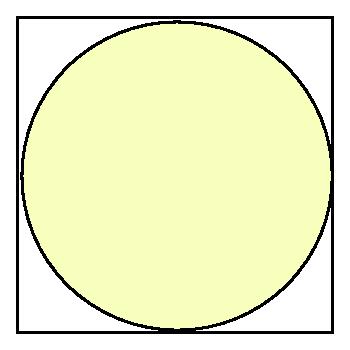
\includegraphics[width=120pt]{test.eps}
\end{center}
\caption{図の例}
\end{figure}
\end{verbatim}

\begin{figure}[ht]
\begin{center}
  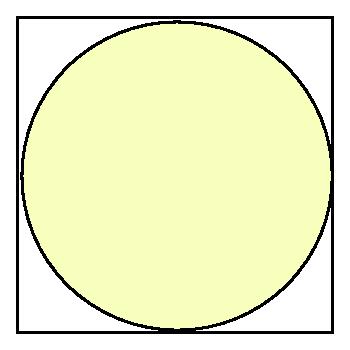
\includegraphics[width=120pt]{test.eps}
\end{center}
\caption{図の例}
\end{figure}


\subsubsection*{(2)表について}
下記のように,tableコマンドとtabularコマンドを使用し,表の下部に対応する
captionを設定してください。

\begin{verbatim}
	\begin{table}[ht!]
\begin{center}
\begin{tabular}{ccc} \hline
&記号 &用法 \\ \hline
<以下略>
\end{tabular}
 \caption{特定の記号の用法}
\end{center}
\end{table}

\end{verbatim}

\begin{table}[ht!]
\begin{center}
\begin{tabular}{ccc} \hline
&記号 &用法 \\ \hline
1 &() &説明・その他付加的に記述する事柄 \\ \hline
2 &``'' &引用箇所の表示 \\ \hline
3 &\textit{Italic} &文中における欧文の書名・誌名 \\ \hline
4 &『 』 &文中における和文の書名・誌名 \\ \hline
\end{tabular}
 \caption{特定の記号の用法}
\end{center}
\end{table}

\subsubsection{文章・表記など}
文章は原則として常用漢字と現代仮名遣いを用いてください。なお,以下の記号
は特定の用法で使ってください(表1参照)。

\begin{description}
 \item[( )] 説明・その他付加的に記述する事柄
 \item[“ ”] 引用箇所の表示
 \item[\textit{Italic}] 文中における欧文の書名・誌名
 \item[『 』] 文中における和文の書名・誌名 
\end{description}

\section{引用・参照文献}
本文中に他の文献からの引用を含める場合には,引用符「`` ''」を
用いて記述してください。また,下記のように,quote環境あるいはquotation環
境を用いることも可能です。
いずれの引用方法でも,末尾に一連番号を付与した上で,出典を記載してくださ
い。形式が一貫している限りで,別の記載方法をとっても構いません。
なお,他の文献の内容・文言を論文中で用いるときには,直接の引用
であるか言い換えた上での内容の利用であるかにかかわらず,出典を
明記する必要があります。



\subsubsection*{例1}
澤田昭夫は良い論文について``よい論文は統一unity,連関coherence,
展開developmentにおいて優れた論文あるいは明確性clarityにおいて優れた論
文''~\cite[p. 19]{澤田}であると述べている。\\\

例1のソースは以下の通りです。
\begin{verbatim}
澤田昭夫は良い論文について``よい論文は統一unity,連関coherence,展開developmentにおいて優れた論文あるいは明確性clarityにおいて優れた論文''~\cite[p. 19]{澤田}であると述べている。
\end{verbatim}

\subsubsection*{例2}
澤田は論文執筆の際に次のようなことが重要だと述べている。
\begin{quote}
論文書きでもっとも大切なのは,問を疑問文の形で切り出すことで,それがレ
 トリックで言う発見・構想です。もっとも大切だというのは,それができれば
 つまり全体を貫く主な問が何であるかを確定することができれば,論文の首尾
 一貫性,統一性を保証する基本的条件が整ったことになるからです。

そのつぎに大切なのは,論文の構成,材料の配置です。その際,肝に銘じなけれ
 ばならないのは,構成・配置の大原則は起承転結ではなく,序・本・結(序と
 本論と結び)だということです\cite[p. 74]{澤田}。
\end{quote}

例2のソースは以下の通りです。
\begin{verbatim}
澤田は論文執筆の際に次のようなことが重要だと述べている。
\begin{quote}
論文書きでもっとも大切なのは,問を疑問文の形で切り出すことで,それがレトリックで言う発見・構想です。もっとも大切だというのは,それができればつまり全体を貫く主な問が何であるかを確定することができれば,論文の首尾一貫性,統一性を保証する基本的条件が整ったことになるからです。

そのつぎに大切なのは,論文の構成,材料の配置です。その際,肝に銘じなければならないのは,構成・配置の大原則は起承転結ではなく,序・本・結(序と本論と結び)だということです\cite[p. 74}{澤田}。
\end{quote}
\end{verbatim}

\subsection{書誌事項の記載形式}
引用・参照文献の書誌事項の記載形式は,原則として以下の通りとします。なお,
以下で{}の部分は,必要に応じて記載する項目です。またイタリック体(斜体
字)を用いる代わりに下線を引いても良いものとします。

LaTeXの場合は,thebibliography環境を用いて,次のように記載します。

\begin{verbatim}
	\begin{thebibliography}{10}
	 \bibitem{澤田}
		 澤田昭夫. 『論文のレトリック』 
		 講談社学術文庫, 講談社, 1983, 330p.
\end{thebibliography}
\end{verbatim}


なお,LaTeX環境でbibtexを文献管理に使用した場合には実現しづらい記載もあ
りますので, 一連番号の形式が一貫している限りで,別の記載方法をとっても
構いません。




\subsubsection{図書の場合}
\noindent{}和:著編者名 『書名』 \{版表示,\} \{出版地,\} 出版社, 出版年, \{総
\bigskip
ページ数,\} 当該部分のページ.\\
洋:author. \textit{title}. \{edition,\} place of publication,
publisher, year, \{total page,\} page.
\begin{quote}
 近藤二郎 『社会科学のための数学入門』 東京経済新報社, 1973,
 p. 37--40.

 Barzun, Jacques and Graff, H. F. \textit{The Modern Researcher.}
 Rev. ed., \\New York, Harcourt, 1970, p. 165.
\end{quote}


\subsubsection{翻訳書の場合}
\noindent{}和:著編者名 『書名』[原書名(イタリックで記載) \{版表示,\}
\{出版地, \} 出版社, 出版年,] 翻訳者名, 出版社, 出版年, \{総
\bigskip
ページ数,\} 当該部分のページ.\\
洋:author. \textit{title of translation} [\textit{original
title}. \{edition,\} place of publication, publisher, year,] name of
translator, place of publication, publisher, year, \{total page,\} page.

\begin{quote}
Varles, Jana ed. 『情報の要求と探索』 [\textit{Information Seeking:
 Basing Services on User's Behaviors.} North Calolina,
 McFarland \& Company, 1987] 池谷のぞみ, 	市古健次, 白石英理子, 田村俊作訳,
 勁草書房, 1993, p. 10.

Schneider, Georg. \textit{Theory and History of Bibliography.}
 [\textit{Handbuch der Bibliographie.} e Aufl., Berlin, Knopt, 1978,]
 tr. by R. R. Shaw, New York, Columbia University Press, 1934, p. 14--15. 
\end{quote}

\subsubsection{編集書の一部(図書形態の論文集の一論文を含む)の場合}
\noindent{}和:当該部分の執筆者名 ``当該部分の題名'' $<$編者名 『書名』 \{版表示,\} \{出版地,\} 出版社, 出版年$>$ \{総
\bigskip
ページ数,\} 当該部分のページ.\\
洋:author. ``\textit{title}''. $<$editor. \textit{book title}, \{edition,\} place of publication,
publisher, year$>$ \{total page,\} page.

\begin{quote}
宮坂広作 ``余暇と社会教育'' $<$碓井正久編著 『社会教育』 第一法規,
 1970$>$ p. 201--203.

Groom, Geofrey. ``Bibliography of older material'' $<$Garvin,
 L. H. ed. \textit{Printed Reference Material.} 2nd ed., London, Library
 Association, 1984$>$ p. 456--501.
\end{quote}


\subsubsection{逐次刊行物掲載記事(雑誌論文を含む)の場合}
\noindent{}和:執筆者名 ``論題名'' 『掲載逐次刊行物名』 vol. XX,
\{no. XX,\} 発行年\{月\}, 当該部分のページ.\\
洋:author. ``\textit{title},'' \textit{name of periodical}, vol. XX,
\{no. xx,\} year\{month\}, page.


\begin{quote}
小野寺夏生 ```Bibliostatistics': 情報現象の統計学的説明'' 『情報管理』
 vol. 21, no. 10, 1979, p. 782--802.

小野寺夏生, 中井浩 ``単純なモデルからのZipfの法則の導入'' 『情報科学技術
 研究集会論文集』 vol. 33, no. 3, 1977, p. 129--138.

Brookes, Bertram C. ``Theory of the Bradford Laws,'' \textit{Journal of
 Documentation,} vol. 33, no. 3, 1977, p. 180--209. 

Nelson, Micheal J. and Tague, Jean M. ``Sprit Size-Rank Models for the
 Distribution of Index Terms,'' \textit{Journal of the American Society
 for Information Science,} vol. 36, no. 5, 1985, p. 283--296.
\end{quote}

\subsubsection{Web上のリソースについて}
Web上のリソースについては,書誌情報の最後に``入手先URL, (アクセス日)''
(``available from (URI), (accessed date)'')を記入します。それ以外の項
目は図書並びに逐次刊行物掲載記事の規定に準じ,入手先の情報から明らかであ
る項目を記述します。

\begin{quote}
 情報メディア学会. 『『情報メディア研究』への各種原稿の投稿について』 入手
 先URI: http://www.jsims.jp/toko.html (参照: 2008--10--27)
\end{quote}

\section{論文の製本について}
論文は必ず,左綴じで製本して提出してください。また,製本後の表紙にも標題ページを記載します。詳細は事務部に確認してください。

製本可能な店は近隣に複数
ありますが,構内では岡田製本店(法文2号館地下),文学部複写センター,生
協コピーセンターが取り扱っています。これらの店は,論文の提出時期は混み合
い製本に時間がかかることがあります。製本の仕上がりが提出期限に遅れないよ
う,充分留意してください。

\section{インタビュー調査および質問紙調査についての注意点について}
インタビューや質問紙調査の対象となった個人や特定組織は論文中では匿名としてください。また,インタビューの書き起こしについては,原則としてインタビュー相手の確認を取ってください。

%-----------------------------参考文献記述エリア---------------------------%
\begin{thebibliography}{10}
 \bibitem{澤田}澤田昭夫. 『論文のレトリック』 
	 講談社学術文庫, 講談社, 1983, 330p.
\end{thebibliography}
%---------------------------------必須エリア-------------------------------%
\end{document}


%----------------------------ファイルはここまで----------------------------%
